\documentclass[journal]{IEEEtran}

% Package to commnet out sections.
\usepackage{comment} 

% Package to make referenzes become ``hyperlinks''
\usepackage{hyperref}

% Package for drawings.
\usepackage{tikz}
\usepackage{caption}
\usepackage{subcaption}

\usepackage{amsmath}

% Get the encoding and language right.
\usepackage[utf8]{inputenc}
% \usepackage[ngerman]{babel}

\usepackage{graphicx}                  % This is needed for including figures and graphics
\usepackage{amssymb}
\usepackage{epstopdf}
\DeclareGraphicsRule{.tif}{png}{.png}{`convert #1 `dirname #1`/`basename #1 .tif`.png}

\title{VP Bericht - Elektronik D}
\author{Julian Viereck - \today}

\begin{document}

\maketitle

\begin{abstract}The here presented experiments give a brief overview on some
important properties of digital circuits. For some properties, it is
described how these are measure. This might serve as a good starting point for
those, that want to understand how digital circuits work.
Problems designing an own circuit are highlighted and solutions are presented.
The importance of understanding the used digital components is emphasized.    
\end{abstract}

\tableofcontents

\section{Introduction}

Over the last years, more and more parts of people's life has become digital.
Some people call this the digital revolution. While the devices get more
packed with functionality and the complexity to build them increases, the root
concept of digital technology stayed the same. There are only two states  still
- 0/"low'' and 1/"high'', which form a single bit, and most digital circuits are
made up of transistors.

The main components of a digital circuits are given by resistors, capacities and
transistors. From these components, logic gates (or just called gates) are
build, that perform a single boolean operation given some input signal (e.g.
take two input signals, perform the AND operation on them and set a output
signal based equal to the result of the AND operation). Gates are then
assembled to so called integrated circuit (short: IC), that can perform more
complex operations.

Logic gates are produced in different ways, which lead to different properties.
Gates with the same properties are grouped into so called logic gate families.
Two important logic gate families are TTL (transistor–transistor logic) and CMOS
(complementary metal–oxide–semiconductor). TTLs are only made up from resistors and
transistors. Typically, they require a supply voltage of 5V. A voltage lower
then 1.8V is interpreted as a "low" signal. The output signal is less then 0.4V
for a low and over 2.4V for a high signal. The big disadvantage compared
to CMOS is the higher power usage. Where TTL uses only bipolar transistors, CMOS also uses
MOSFETs. The voltage for the power supply can range from 3V to 30V. The voltage
ranges detected as high/low signal depends on the power supply voltage.

The following experiments will concentrate on analysing some of the properties
of CMOS ICs. This will start by determining the performed operation of some ICs
and their propagation delay. Next, a pulse generator is build and examined.
Finally, a simple bit shift logic is presented, which was self designed and some
of the issues going with the self designing are explained.

\section{Experiment: Simple Logic Gate}

\subsection{Samples and measurement setup}

\begin{figure}[h!]
  \centering
   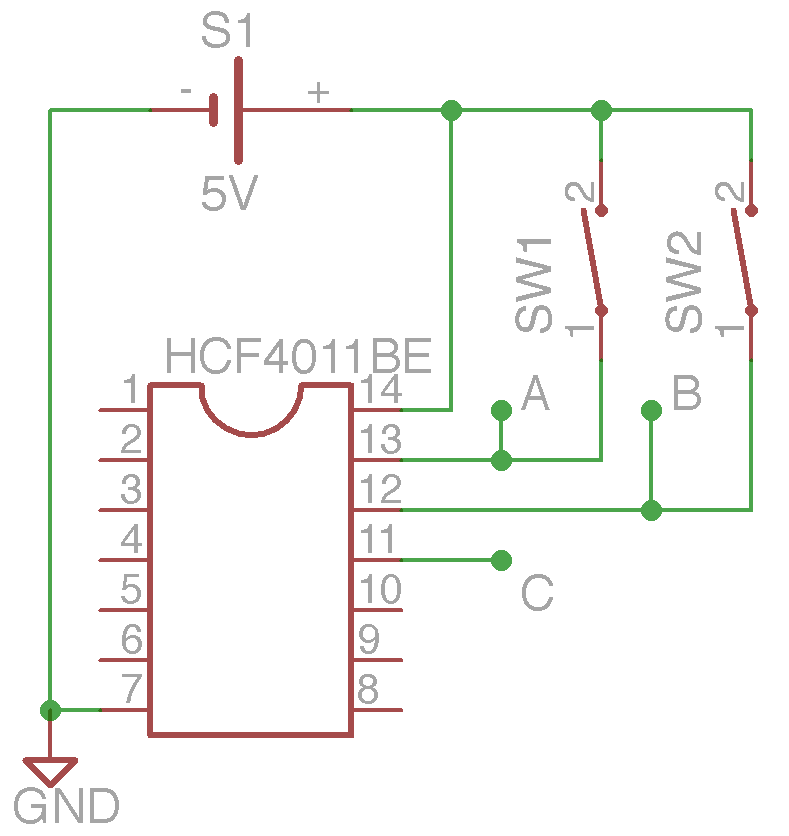
\includegraphics[]{boards/truth.png}
   \caption{Circuit diagram to measure truth table.}
   \label{fig:truth_circuit}
\end{figure}

The circuit was setup as shown in figure \ref{fig:truth_circuit}. Based on the
different input signals at A and B, different values for the output signal C
were measured using a oscilloscope. As for the ICs, a HCF4001BE and HCF4011BE
were used.

To measure the propagation delay, input signal A was connect to a square wave
voltage generator. Input signal B was connected to ground. The IC HCF4001BE
was used for this measurement. The voltage of the generator was set to 2.9V and
the frequency to 1Hz. The voltage was chosen, such that a slightly lower
voltage was detected as a ``low" input signal. The input signal A and output
signal C was visualized using a oscilloscope. The oscilloscope's trigger signal was connected to the voltage generator.

\subsection{Results}

\begin{figure}
	\centering
	\begin{tabular}{c c | c || c c | c}
 		 \multicolumn{2}{c}{4011}
  		 \multicolumn{5}{c}{4001} \\
		  A & B & C & A & B & C \\ \hline
		  0 & 0 & 1 & 0 & 0 & 1 \\
		  0 & 1 & 1 & 0 & 1 & 0 \\
		  1 & 0 & 1 & 1 & 0 & 0 \\
		  1 & 1 & 0 & 1 & 1 & 0 \\
	\end{tabular}
	\caption{Truth table measuring IC HCF40011BE and HCF4001BE.}
	\label{tab:truthtable} 
\end{figure}

 \begin{figure}
   \centering
  \begin{tikzpicture}
    \node[anchor=south west,inner sep=0] at (0,0)
    {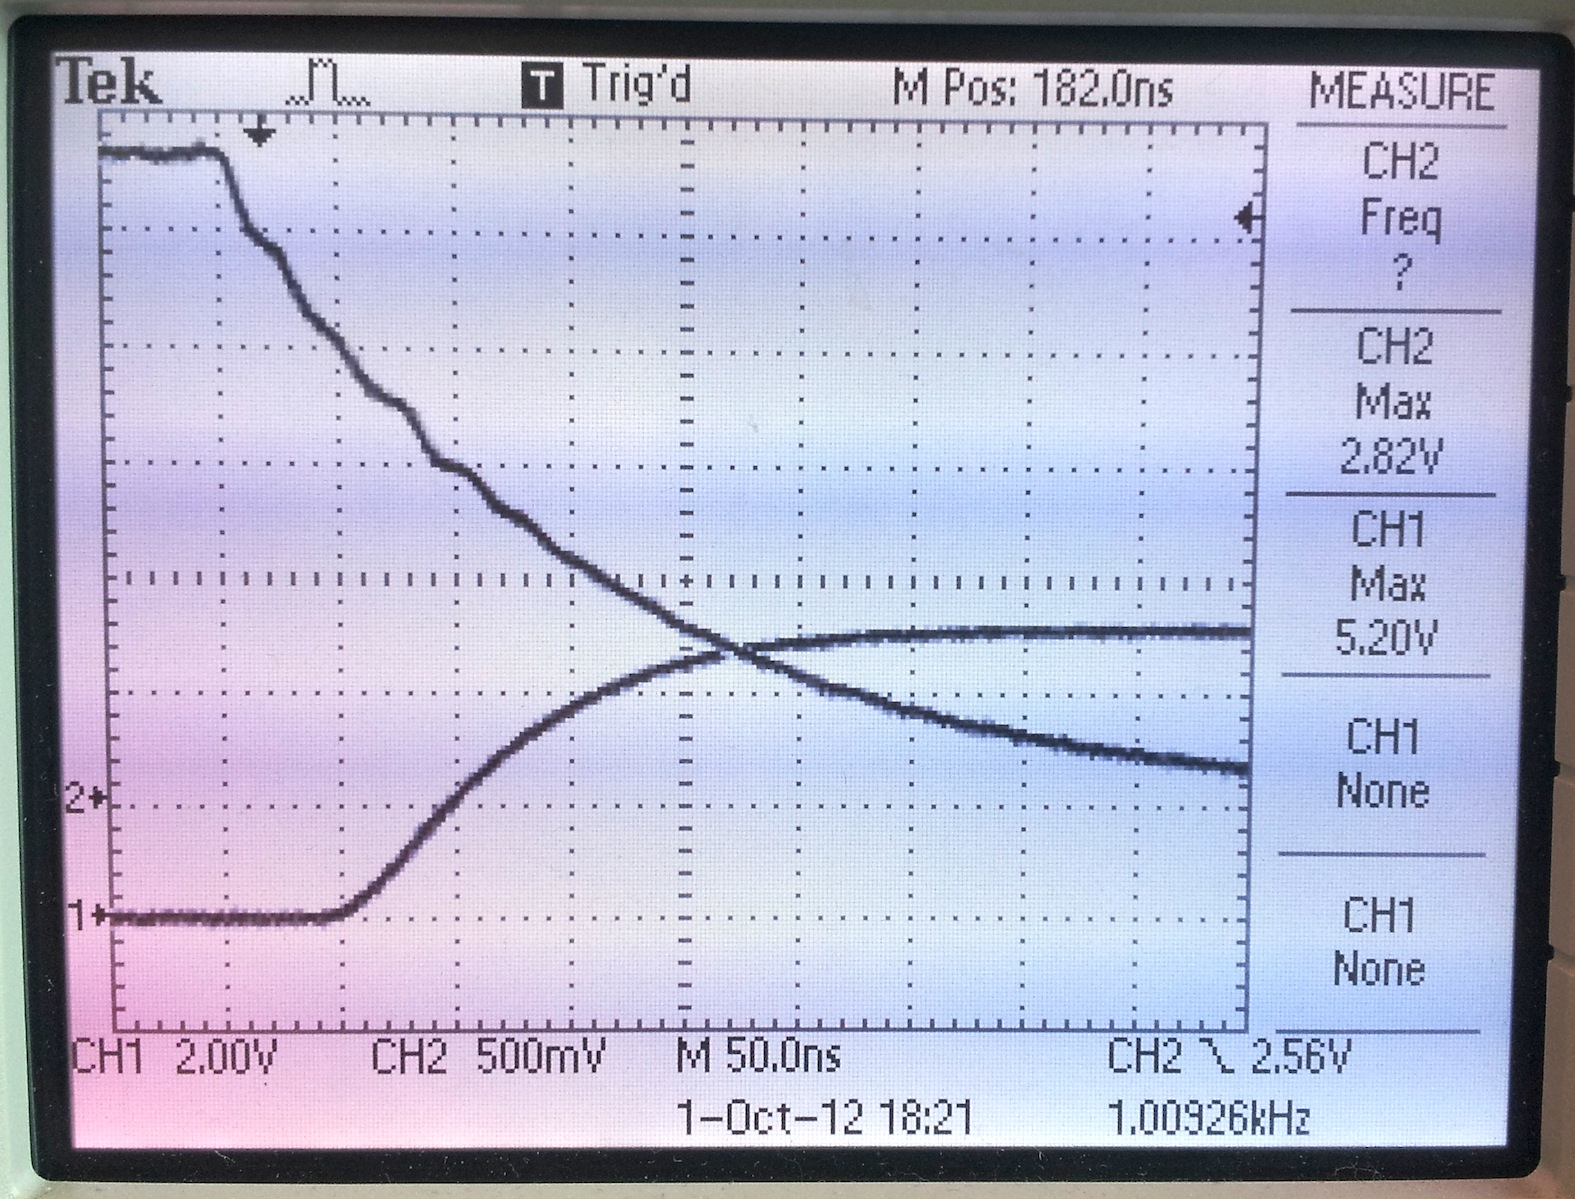
\includegraphics[width=\columnwidth]{img/delay.jpg}};
    \draw[color=red] (1.2,1.1) -- (1.2,6);
    \draw[color=red] (1.9,1.1) -- (1.9,6);
    \path[<->] (1.2, 3) edge node[below]{$\approx 50ns$} (1.9,3);
    \path[<-] (3.3, 3.8) edge node[near end, align=left, right]{Input signal A}
    (4,5);
    \path[<-] (3.3, 2.5) edge node[near end, align=left, right]{Output signal C}
    (4,1.2);
  \end{tikzpicture}
  \caption{Propagation delay measurement.}
  \label{fig:propdelay}
\end{figure}

For different input signals A and B the truth-table was measured as
shown in table \ref{tab:truthtable}.

The propagation delay was measured to be around 50ns as seen in figure
\ref{fig:propdelay}.

\subsection{Analysis and Discussion}

Based on the measurements, the IC HCF4001BE seems to be a logic NOR gate,
whereas the IC HCF4011BE seems to function as a NAND gate. This fits with the
specified functionality of the gates.

Looking up the propagation delay from the data sheet, it is said to be typically
around 40ns and up to 75ns. This fits with the here measured delay.

\section{Experiment: Pulse Generator}

Pulse generators create rectangular, periodic voltage signals. In
this experiment, such a generator was build and its properties examined. 

\subsection{Samples and measurement setup}

\begin{figure}[h!]
  \centering
   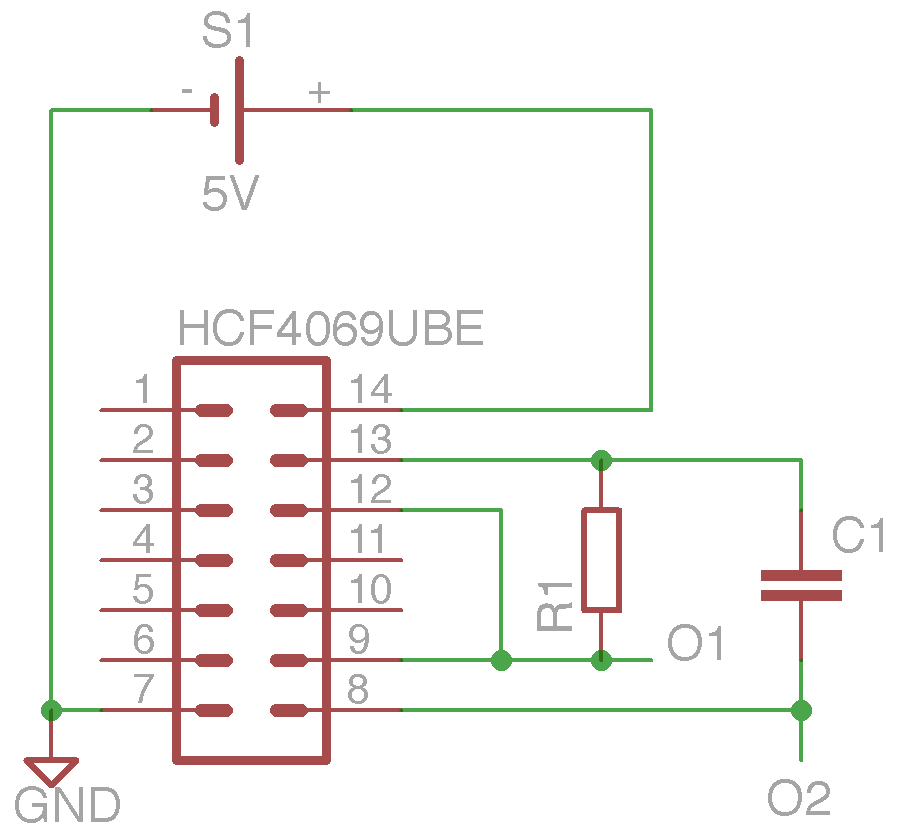
\includegraphics[]{boards/astabil_multivibrator.png}
   \caption{Circuit diagram of astable multivibrator.}
   \label{fig:am_board}
\end{figure}

The circuit was assembled as shown in figure \ref{fig:am_board}. Here, the IC
HCF4069UBE was used, which contains six NOT gates. The voltage difference
between the output signals $O1$, $O2$ and the ground was quantified using an
oscilloscope. This also allowed to visualize and measure the period of the
oscillations.
Different values for the resistance $R1$ and the capacity $C1$ were chosen and
the resulting period of the voltage signals recorded.

\subsection{Functionality explanation}

\begin{figure}[h!]
  \centering
   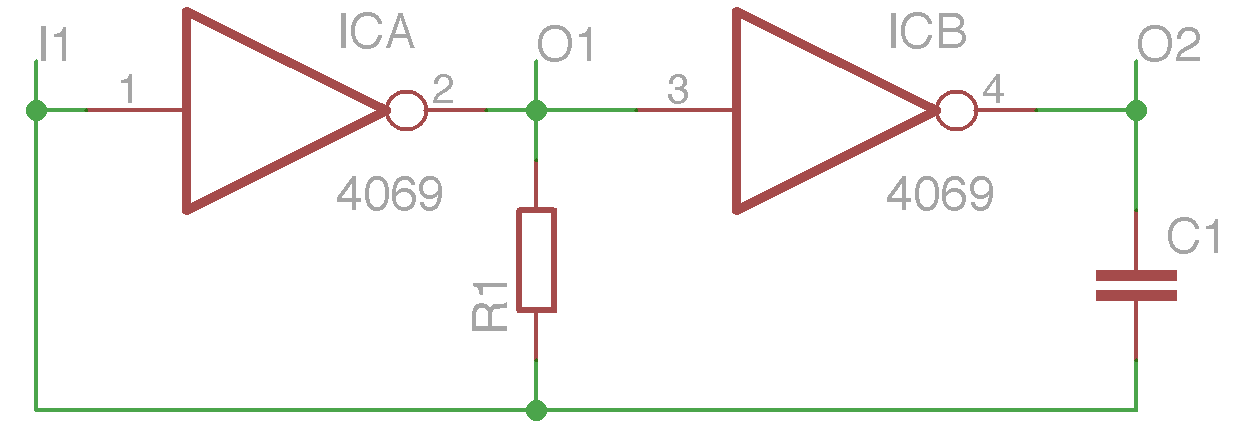
\includegraphics[]{boards/am_overview.png}
   \caption{Schematic drawing of the astable multivibrator circuit.}
   \label{fig:am_scheme}
\end{figure}

A schematic drawing of the circuit is presented in figure \ref{fig:am_scheme}.
The explanation follows the one given in \cite{book_dg}. Let's assume the
voltage at $O1$ is set to be \emph{high} and the capacitor is uncharged. Due to
the \emph{high} signal at $O1$, the signal at $O2$ is \emph{low} (remember ICA
and ICB are NOT gates).
The capacitor is charged over the resistance $R1$. At some point, the voltage at
$I1$ is high enough, such that the input signal of $ICA$ is recognized as \emph{high}. This causes the
signal at $O1$ to become \emph{low} and therefore the signal at $O2$ to be
\emph{high}. The charged capacitor discharges, which keeps the \emph{high}
signal at the $I1$ input for some time until the voltage on the capacitor is too
low, such that the signal at $I1$ is recognized as a \emph{low} signal. The
signal at $O1$ becomes a \emph{high} one and things start over again.

\subsection{Results}

\begin{figure}
	\begin{subfigure}[b]{\columnwidth}
		\centering
		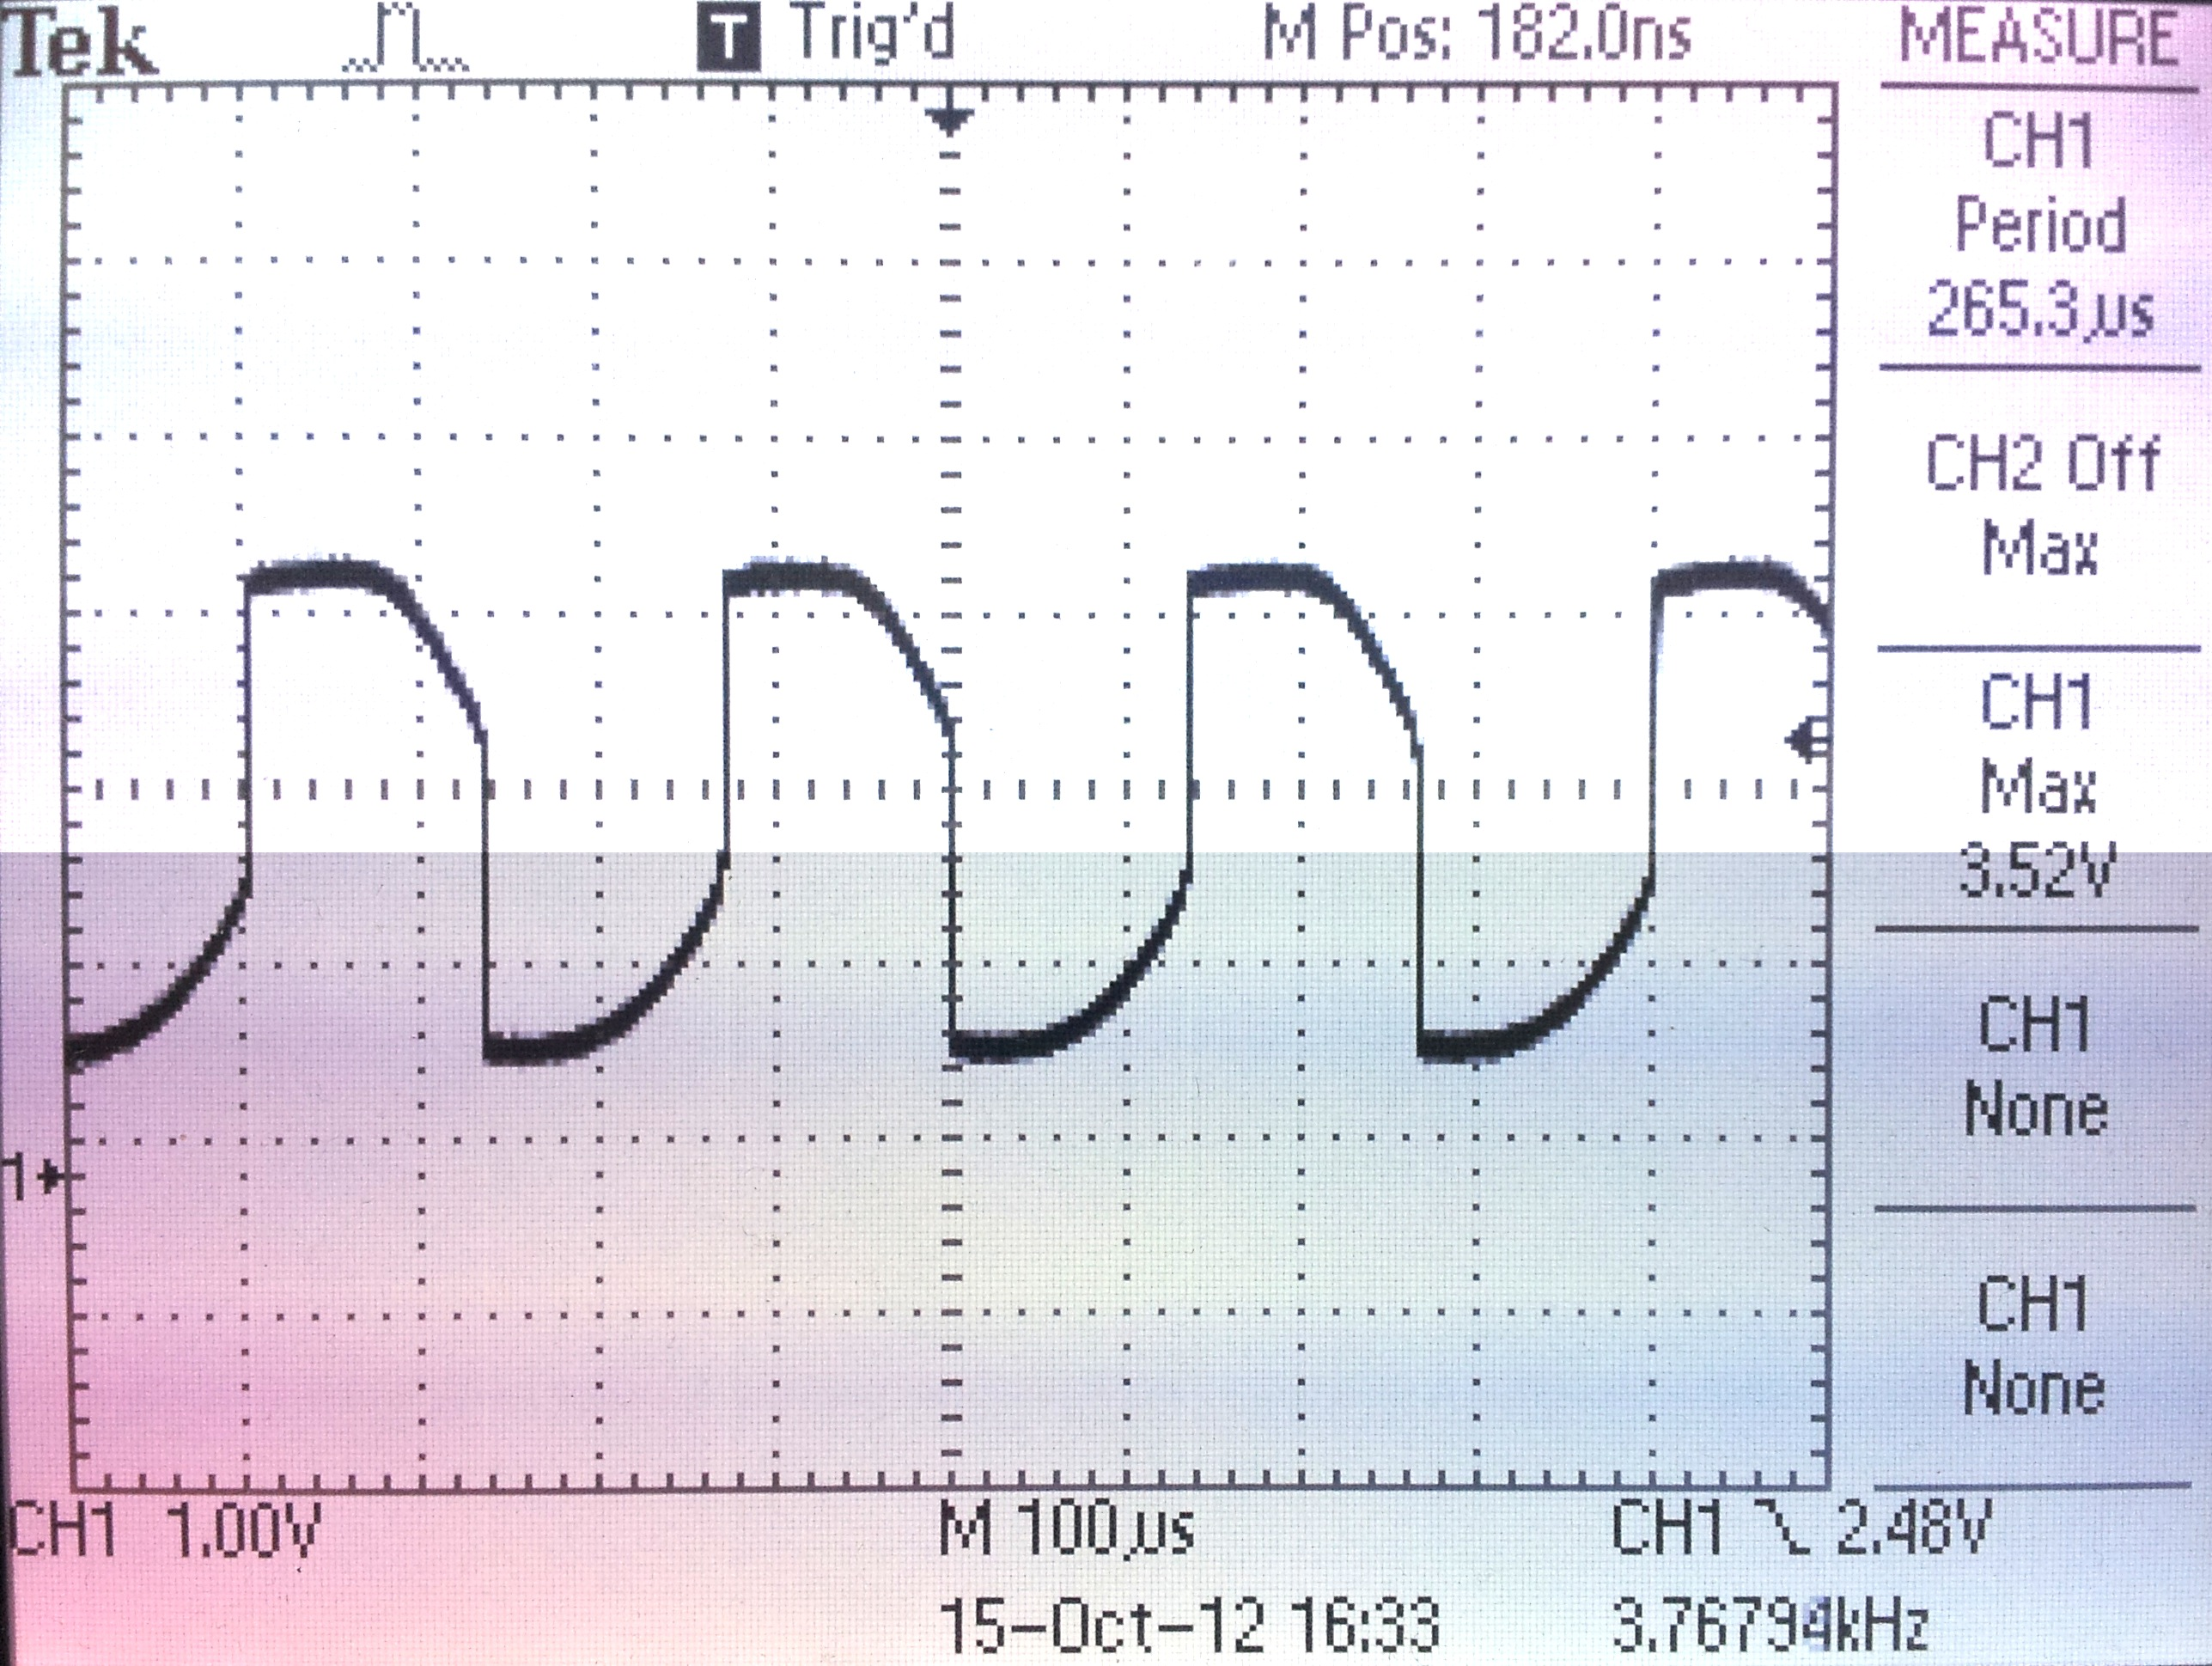
\includegraphics[width=\textwidth]{img/am_o1_timing.jpg}
	\end{subfigure} \\
	\begin{subfigure}[b]{\columnwidth}
		\centering
		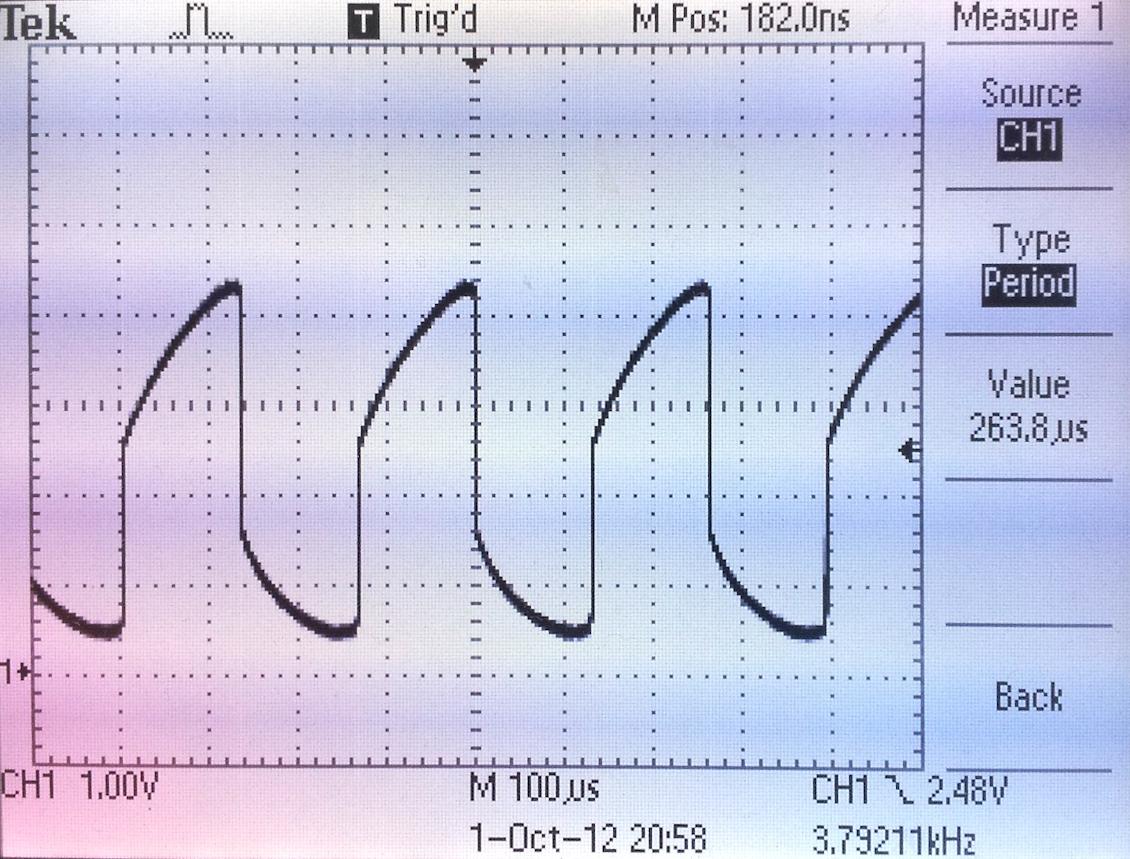
\includegraphics[width=\textwidth]{img/am_o2_timing.png}
	\end{subfigure}
	\caption{Up: voltage difference at O1; bottom: voltage difference at O2. Both
	as function of time.}
	\label{fig:am_timing}
\end{figure}

\begin{comment}
\begin{figure}
  \centering
   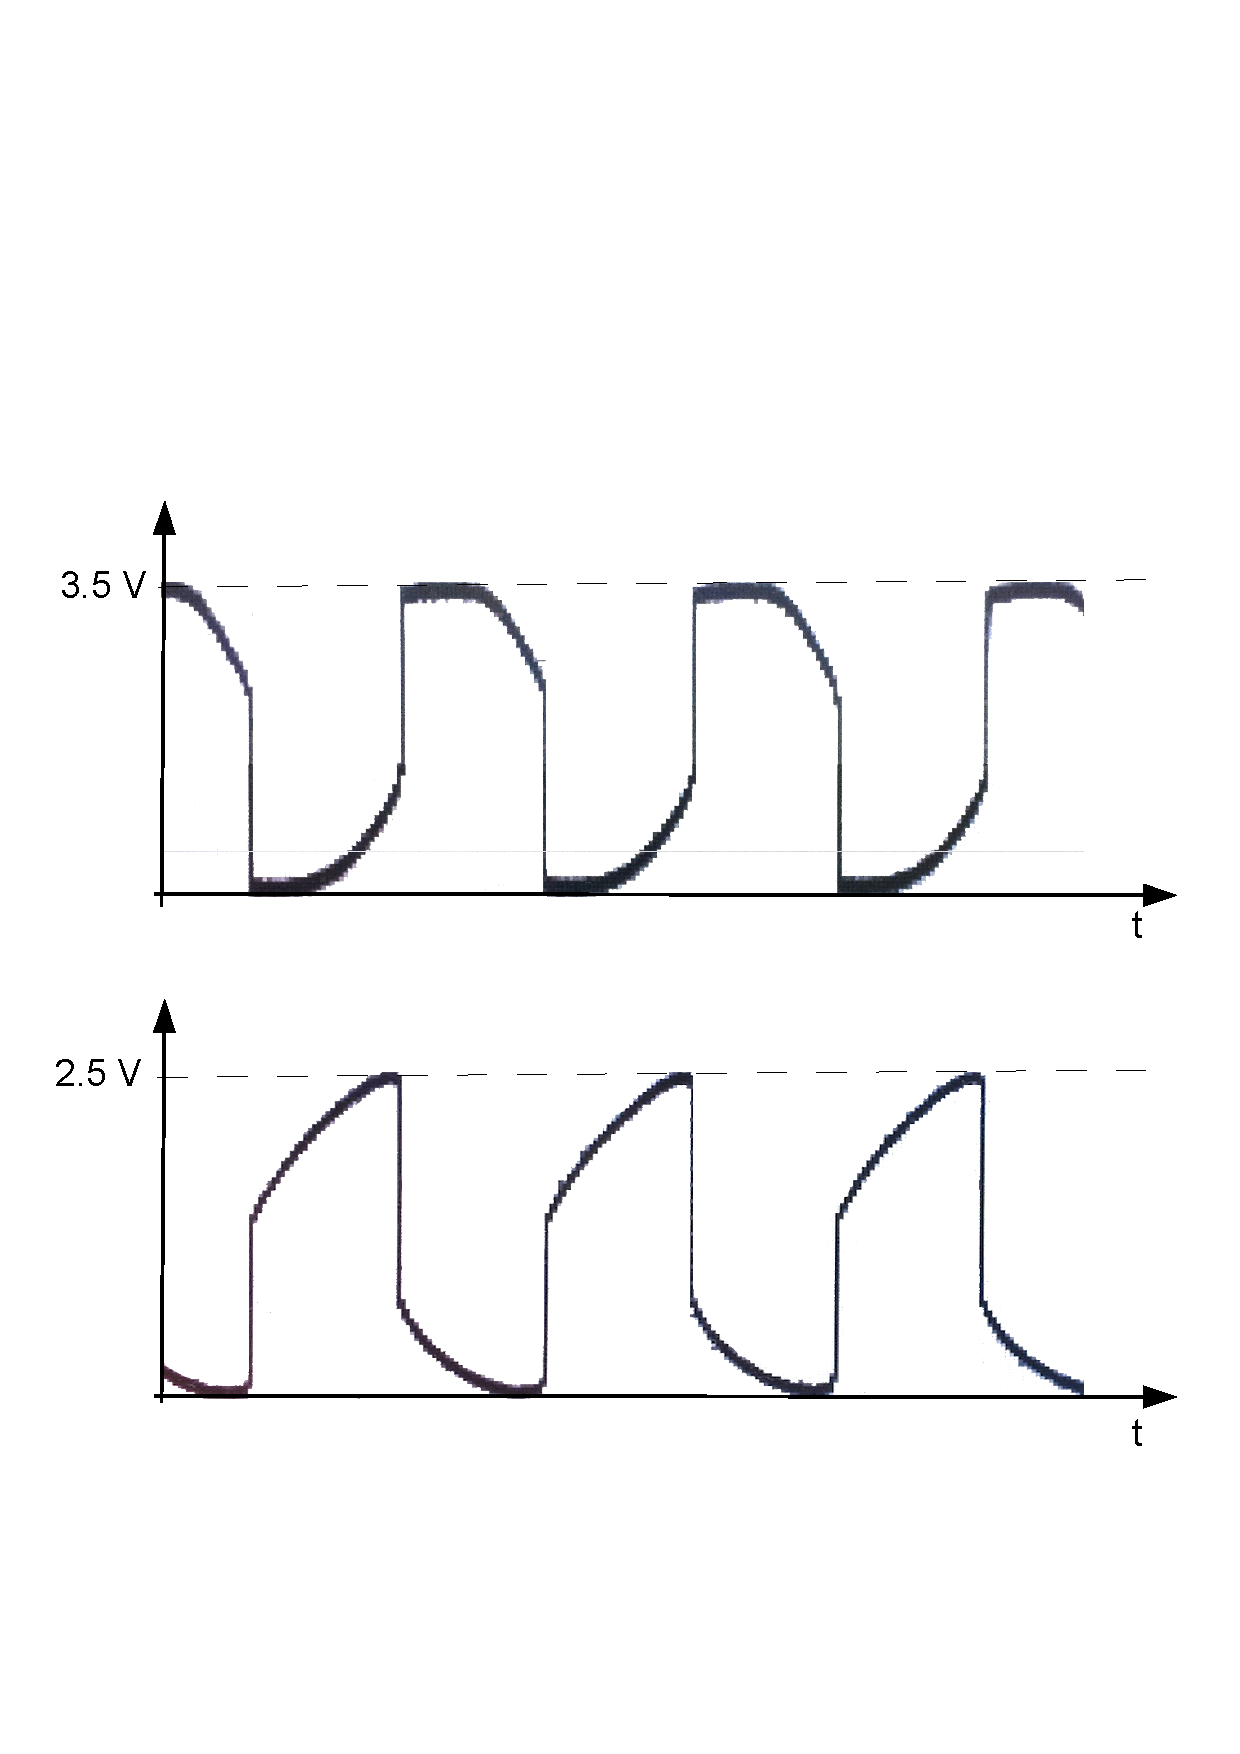
\includegraphics[trim=10mm 50mm 1mm 90mm, clip,
   width=\columnwidth]{img/am_timing.pdf}
   \caption{Timing diagram. Up: Voltage signal at $O1$; bottom: Voltage signal
   at $O2$.}
   \label{fig:am_timing}
\end{figure}
\end{comment}

\begin{figure}
  \centering
   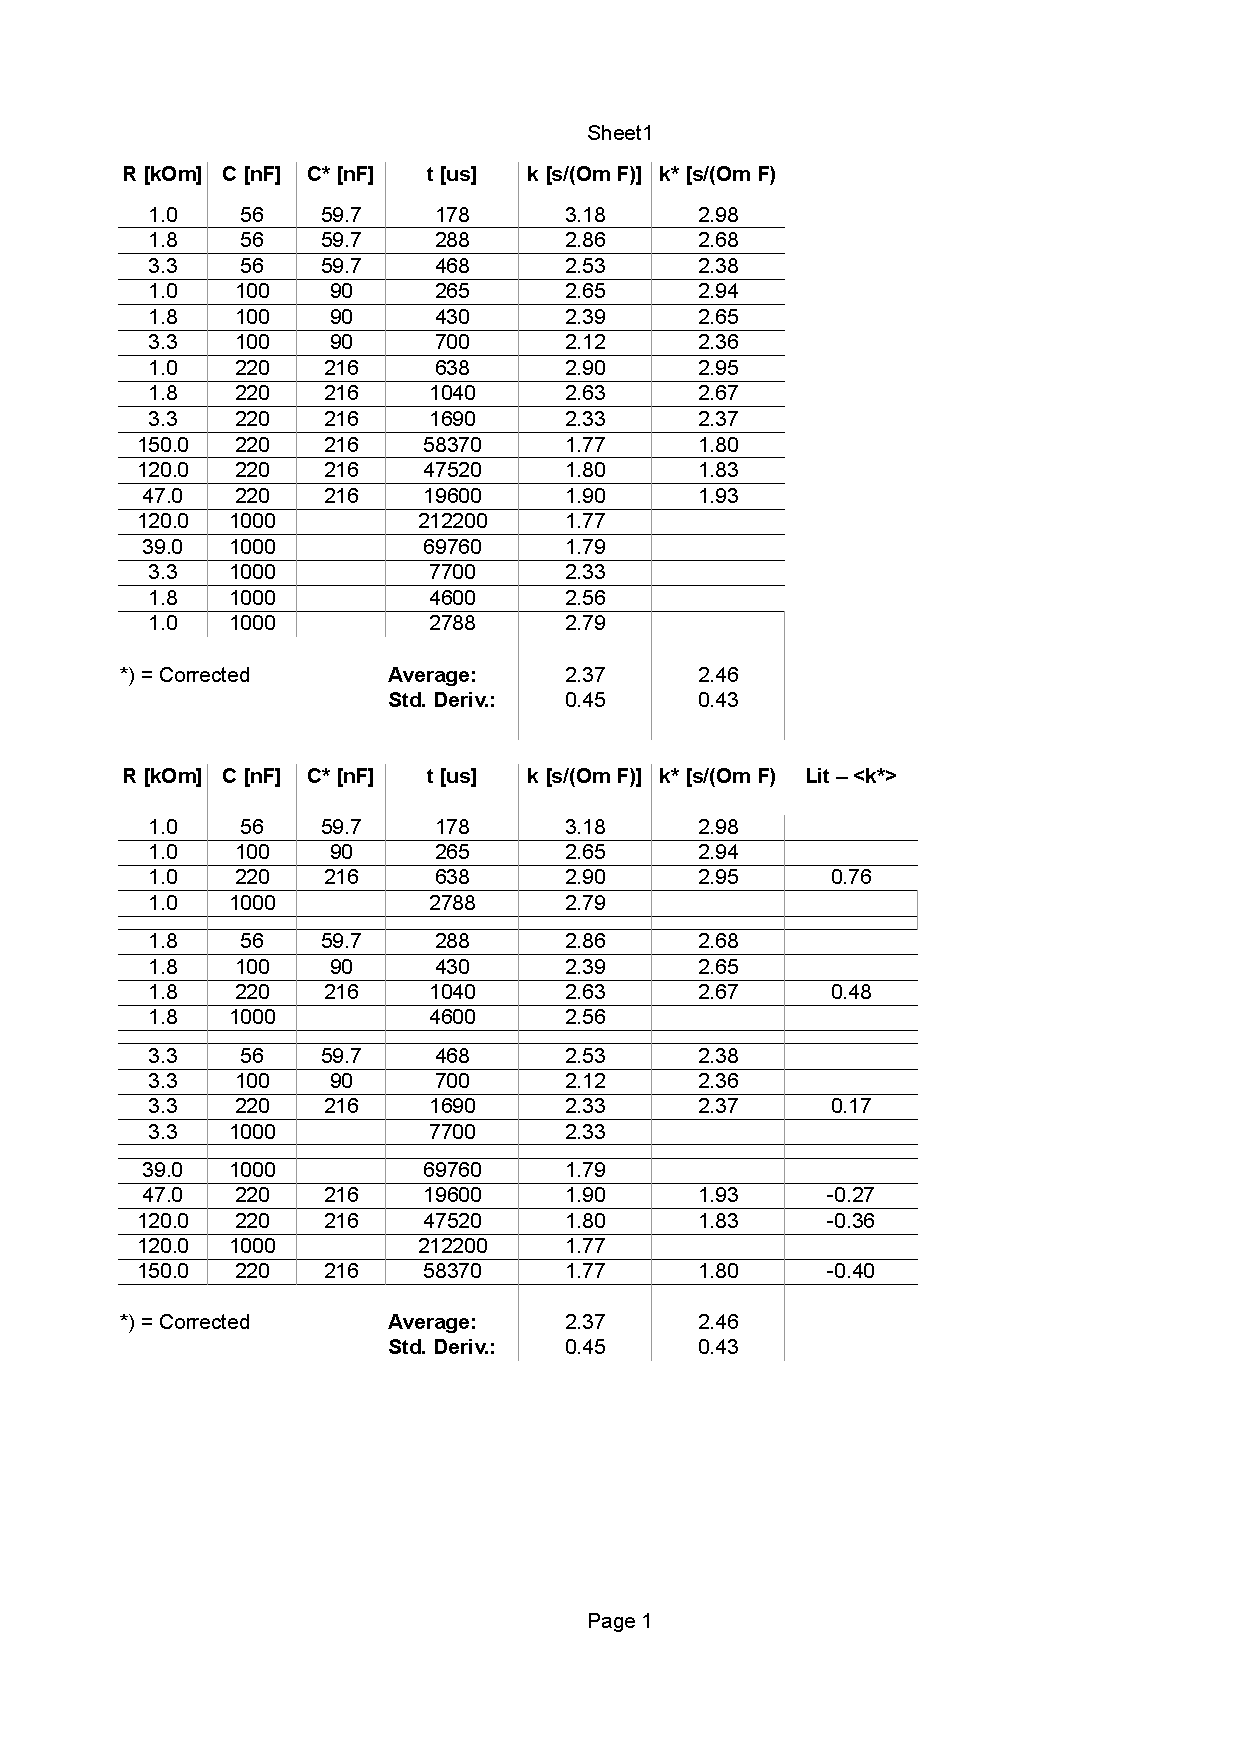
\includegraphics[trim=20mm 63mm 55mm 130mm, clip,
   width=\columnwidth]{results/am_data.pdf}
   \caption{Measurement of period time $t$ as function of resistance $R$ and
   capacity $C$.}
   \label{fig:am_result}
\end{figure}


The time diagram for the voltage at $O1$ and $O2$ is visualized in figure
\ref{fig:am_timing}. In table \ref{fig:am_result} different period times $t$ due 
to different choices of resistance $R$ and capacity $C$ are listed. The values
for the resistances and the capacities used contain a manufacturing
error of roughly up to $10\%$. Some of the capacities were more precise
measured and are listed in the $C*$ column.

\subsection{Analysis and Discussion}

The k-value is defined as

\begin{equation}
	k = \frac{t}{R \cdot C}
	\label{eq:k}
\end{equation}

where $t$ is the period time, $R$ is the resistance of the resistor
\em{R} and $C$ is the capacity of the capacitor \em{C}. Based on the
measurements, the k-values are computed in the $k$
column of table \ref{fig:am_result}. For the more precisely measured
capacities $C*$, the k-value $k*$ was computed using the $C*$ value.

As mentioned in \cite{book_dg}, the relation between $t$ and the other
quantities is given by

\begin{equation}
	t = 2RC\ln(3) \approx 2.2RC
\end{equation}

which gives the value of $k$ using equation (\ref{eq:k}) as

\begin{equation}
	k = 2~\ln(3) \approx 2.2
	\label{eq:k_lit}
\end{equation}

The average values of $k$ and $k*$ given in table \ref{fig:am_result} match with the expected values for k. Using the standard derivation of the
average as an indicator for the uncertainty of the here computed $k$ and $k*$
values, the literature value is within the range of average +- standard derivation.
However, the standard derivation is larger then 1/10 of the average value.
 This indicates a high uncertainty in the measured quantities.

\begin{figure}
  \centering
   \includegraphics[trim=50mm 90mm 45mm 125mm, clip,
   width=\columnwidth,page=2]{results/am_data.pdf}
   \caption{Plot of error comparing literature value to computed value for k* at
   C = 200nF.}
   \label{fig:am_plot}
\end{figure}

The last column $Lit - \<k*\>$ holds the difference between the literature value
(\ref{eq:k_lit}) and the calculated $k*$ value and therefore a simple error
estimation. A plot of these errors for $C = 200\text{nF}$ is shown in figure
\ref{fig:am_plot}. The x-axis is plotted logarithmically. The shape of the curve
suggests a exponential relation between $R$ and the error. As the $k*$ values
are roughly the same for different choices of $C$, this might be an indication,
that the error is mostly related to the choice of the resistance. The reason for
this correspondence remained unclear to the author.

\section{Experiment: Self Build Digital Circuit}

In the last experiment, a shift operation was designed and implemented. For
simplicity, the shifter presented is made up of only two input signals and zero
or one shift of the bits to the left. Written as a programming expression, this
corresponds to:

\begin{equation}
	\{0, 1, 2, 3\} ~ \texttt{<<} ~ \{0, 1\}
\end{equation}

where the numbers in brackets represent all possible values. The result of the
calculation was visualized to the user using three LEDs.

\subsection{Samples and measurement setup}

To get an idea how the circuit should be setup, the required logical operations
were determined as:

 
\begin{equation}
\begin{tabular}{ c l }
      \text{LED1} &= I1 \wedge \lnot S \\
		\text{LED2} &= (I2 \wedge \lnot S) \vee (I1 \wedge S) \\
		\text{LED3} &= (I2 \wedge S)
\end{tabular}
	\label{eq:}
\end{equation}
	
where $I1$, $I2$ are the two input signal for the number to shift (the
number to shift is represented in binary form), $S$ indicates if a shift should
happen (if high, do a shift on the input $I1$, $I2$) and LED\{1,2,3\} are the LEDs
showing the result of the operation.

\begin{figure}[h!]
  \centering
   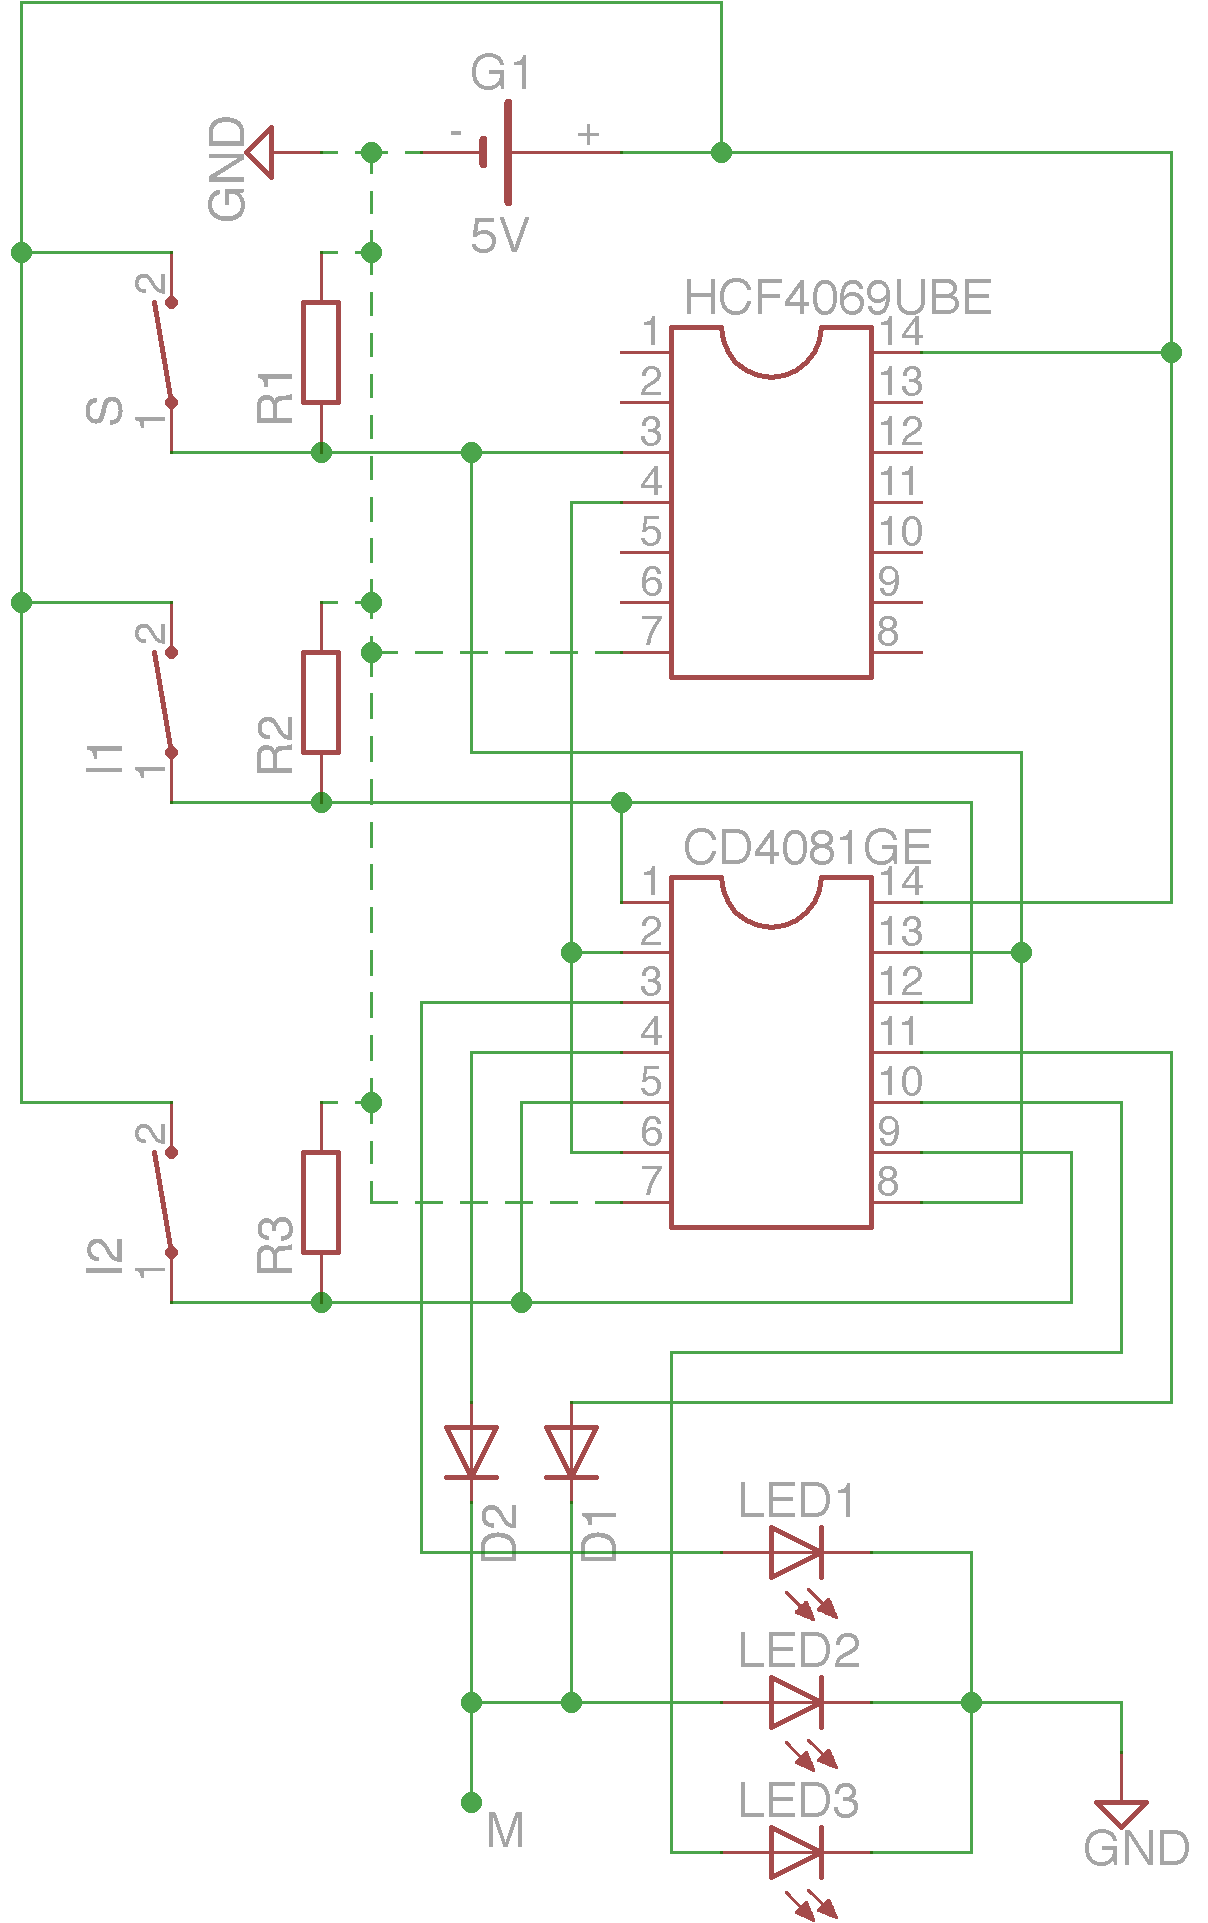
\includegraphics[]{boards/shifter.png}
   \caption{Self designed bit shifter circuit.}
   \label{fig:shifter}
\end{figure}

After looking up the required components, the circuit was sketched out as shown
in figure \ref{fig:shifter}. The four AND operations were covered using the IC
CD4081GE, the NOT operation using the IC HCF4069UBE, the OR operation was done
by ``just'' connecting two wires at first place. In the first draft of
the circuit the components R\{1, 2, 3\} and D\{1, 2\} were left
out. The reasoning for adding them is provided in the ``Analysis and
Discussion'' section.

To determine the propagation delay, input S was connected to a square
wave generator running at 1kHz and 5V. The input I2 was opened/set to a ``low''
signal and the I1 input was closed/set to a ``high'' signal. The voltage
difference at LED2 compared to GND was measured by attaching an oscilloscope at
M.

\subsection{Results} 

\begin{figure}
  \centering
   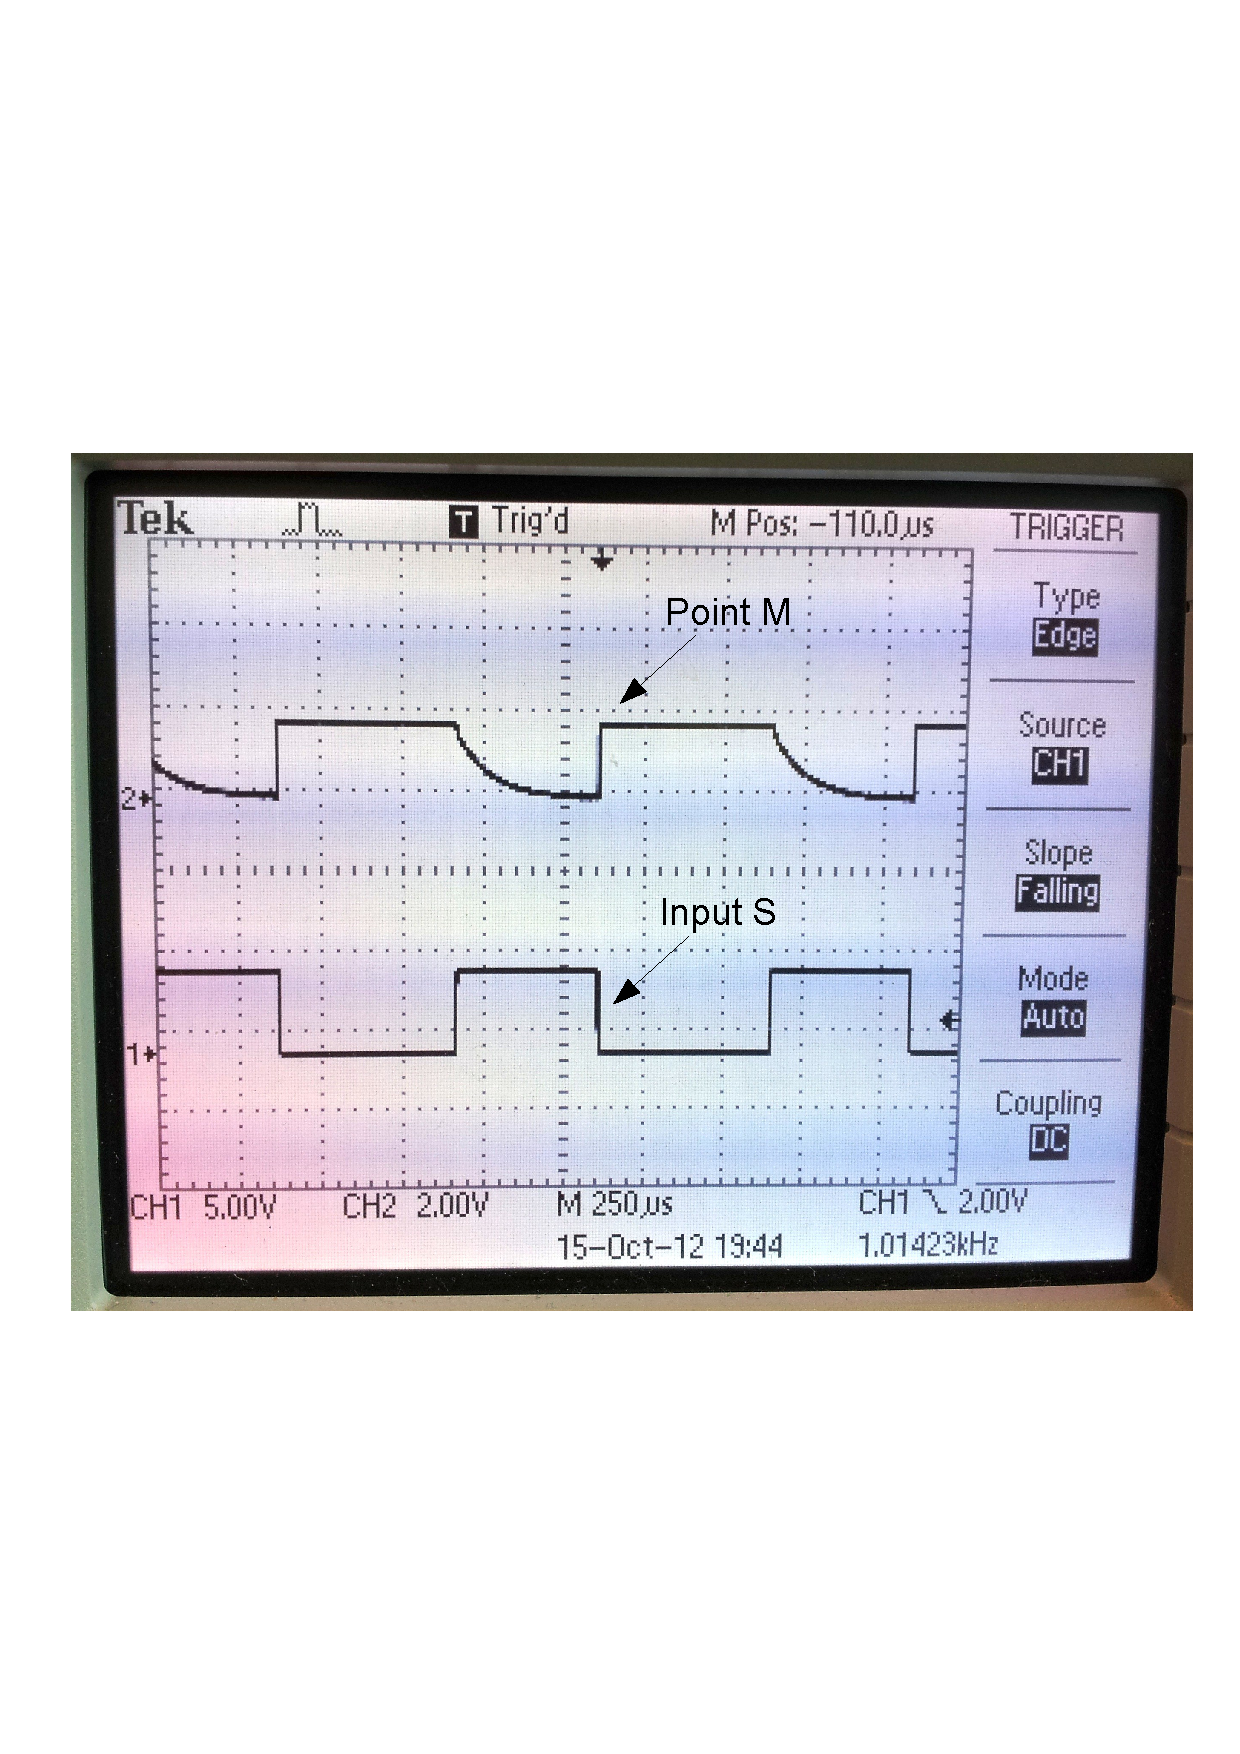
\includegraphics[trim=15mm 75mm 10mm 80mm, clip,
   width=\columnwidth]{img/shift_volt1.pdf}
   \caption{Voltage difference at point M and input S compared to GND using
   D1=1N4148PH.}
   \label{fig:signal_m1}
\end{figure}

The output signals of the AND gates was oscillating. The LED2 was
shining only very little.

After fixing these issues (see next section), the signal at the
output M was measured and is shown in figure \ref{fig:signal_m1}.

\subsection{Analysis and Discussion}

The oscillation of the AND gate output signal was due to not well set ``low''
signal at the gates' inputs. The first draft missed out the resistors R\{1, 2,
3\}.
It was assumed, that no input signal at a gate results in a ``low'' signal.
For the here used AND gates, the ``low'' signal needed to be explicit connected to 
the ground. By using the resistors, the gates detected a ``high'' signal
for closed switches. At the same time for opened
switches the wire was set to a ``low'' signal as the resistors connected the
wire to the GND.
The resistors were chosen to be $100\Omega$. The choice of $18\Omega$ worked
as well, but the resistors got very
hot and therefore got replaced by the $100\Omega$ ones. 

``Just'' connecting the wires for LED2 turned also out to be a bad idea.
A ``high'' signal at one of the wires was attenuate by the ``low'' signal of
the other wire. Therefore, the two diodes D1 and D2 were added. This made the
LED2 shine much brighter.

With these two changes, the shifter circuit was operating as planed.

The wave form measured for the point M in figure \ref{fig:signal_m1} was not
expected. It looks like a discharge curve seen in a resistor-capacity circuit.
However, the shifter circuit doesn't
have any capacities at first sight. Replacing the diode D1 with a wire made the
wave become rectangular. This indicated a correlation between the unexpected
wave shape and the used diode.

\begin{figure}
  \centering
   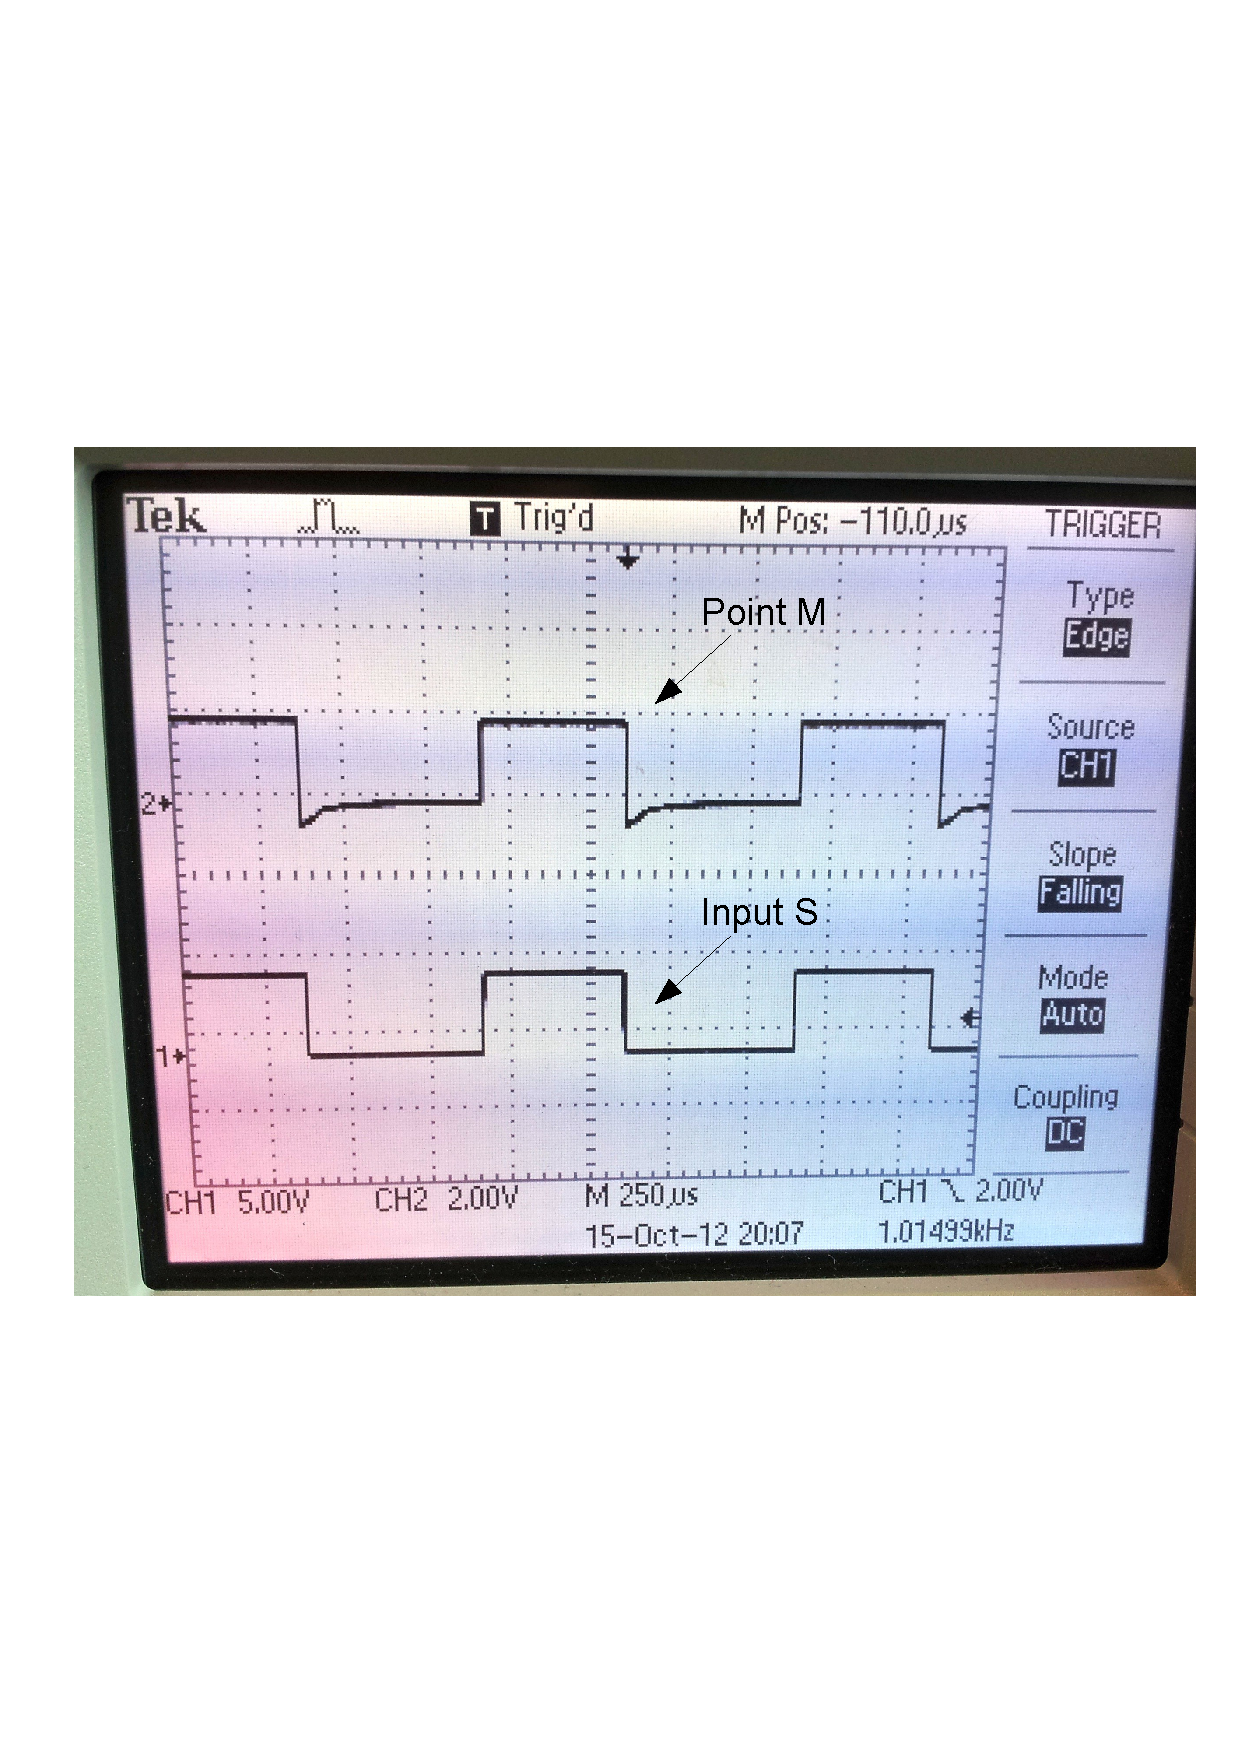
\includegraphics[trim=15mm 75mm 10mm 80mm, clip,
   width=\columnwidth]{img/shift_volt2.pdf}
   \caption{Voltage difference at Point M and Input S compared to GND using
   D1=1N40058912}
   \label{fig:signal_m2}
\end{figure}

The initially used diodes were of the type 1N4148PH. Replacing D1 with the type
1N40058912 changed the waveform's shape as seen in figure \ref{fig:signal_m2}.

\begin{figure}[h!]
  \centering
   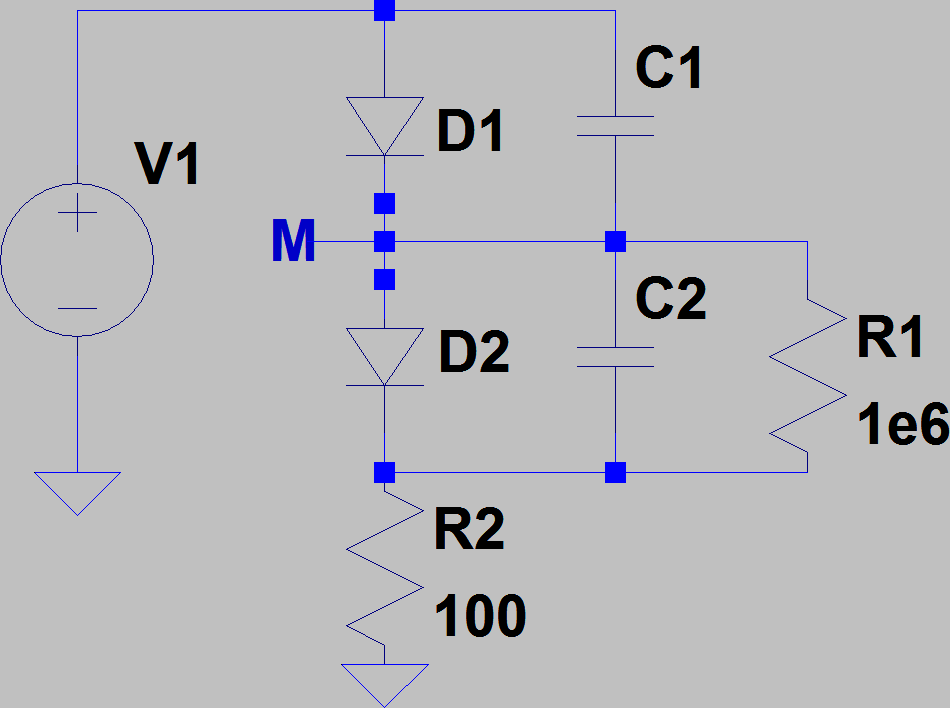
\includegraphics[width=\columnwidth]{img/sim_circuit.png}
   \caption{Reduced circuit used for simulation.}
   \label{fig:signal_model}
\end{figure}

\begin{figure}
	\begin{subfigure}[b]{\columnwidth}
		\centering
		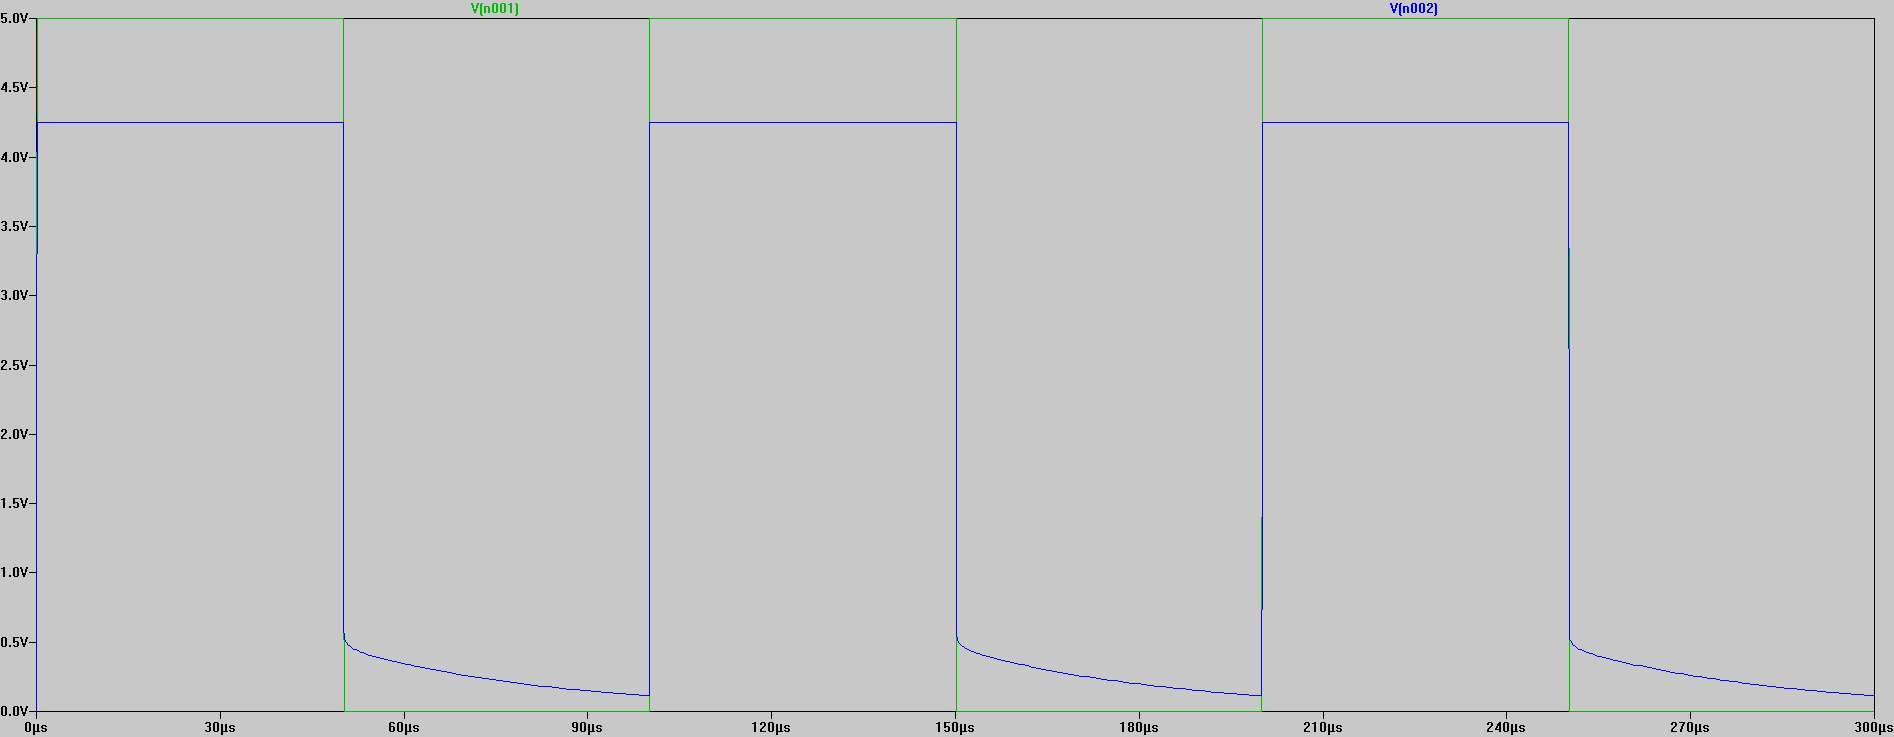
\includegraphics[width=\textwidth]{img/sim_1.png}
		\caption{C1 = 0.9pF, C2 = 35pF}
	\end{subfigure} \\
	\begin{subfigure}[b]{\columnwidth}
		\centering
		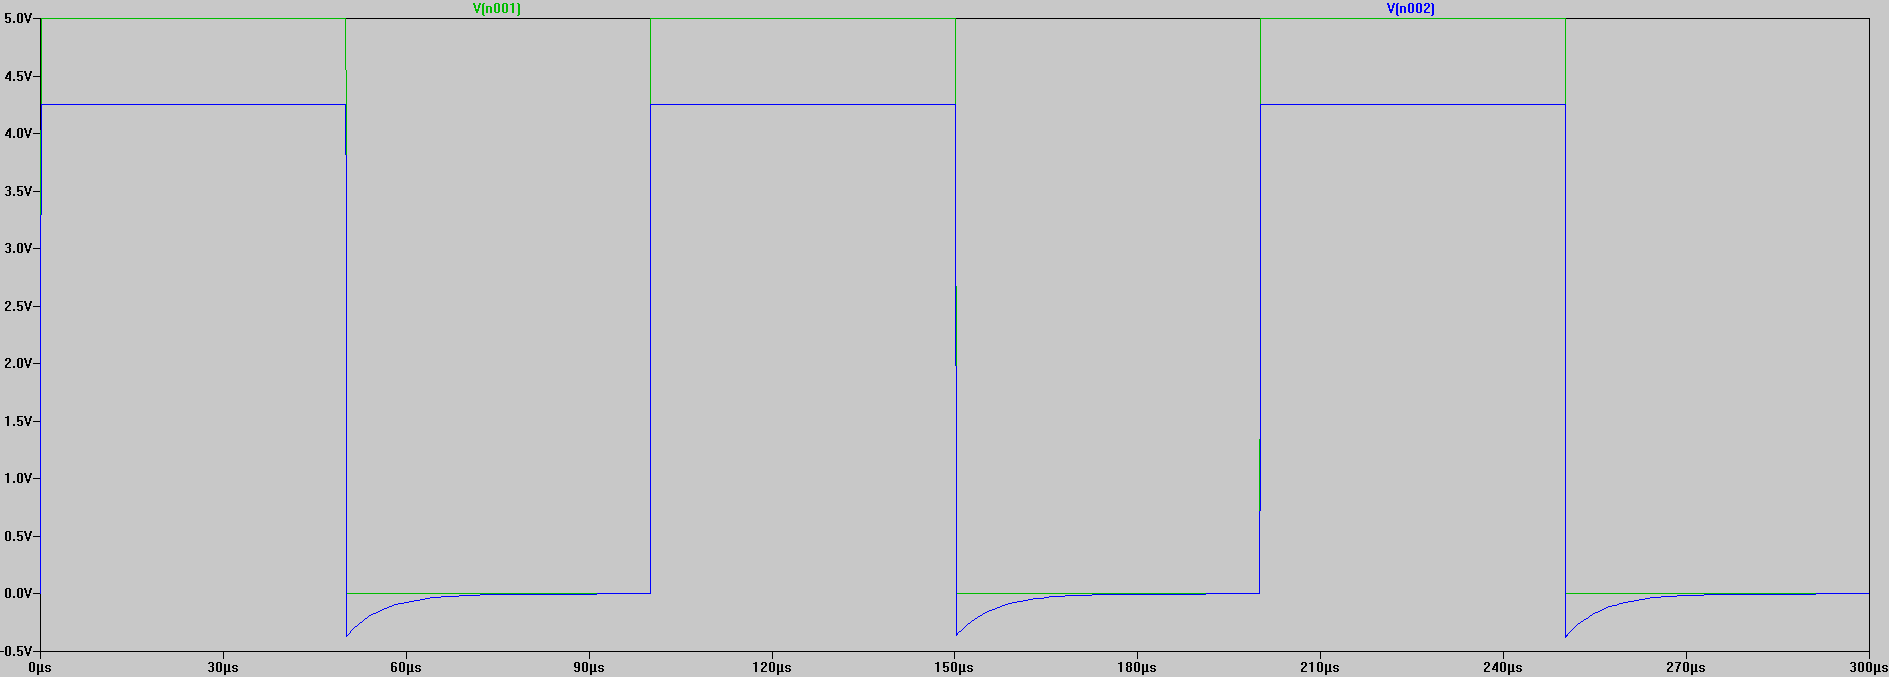
\includegraphics[width=\textwidth]{img/sim_2.png}
		\caption{C1 = 5pF, C2 = 1pF}
	\end{subfigure} \\
	\begin{subfigure}[b]{\columnwidth}
		\centering
		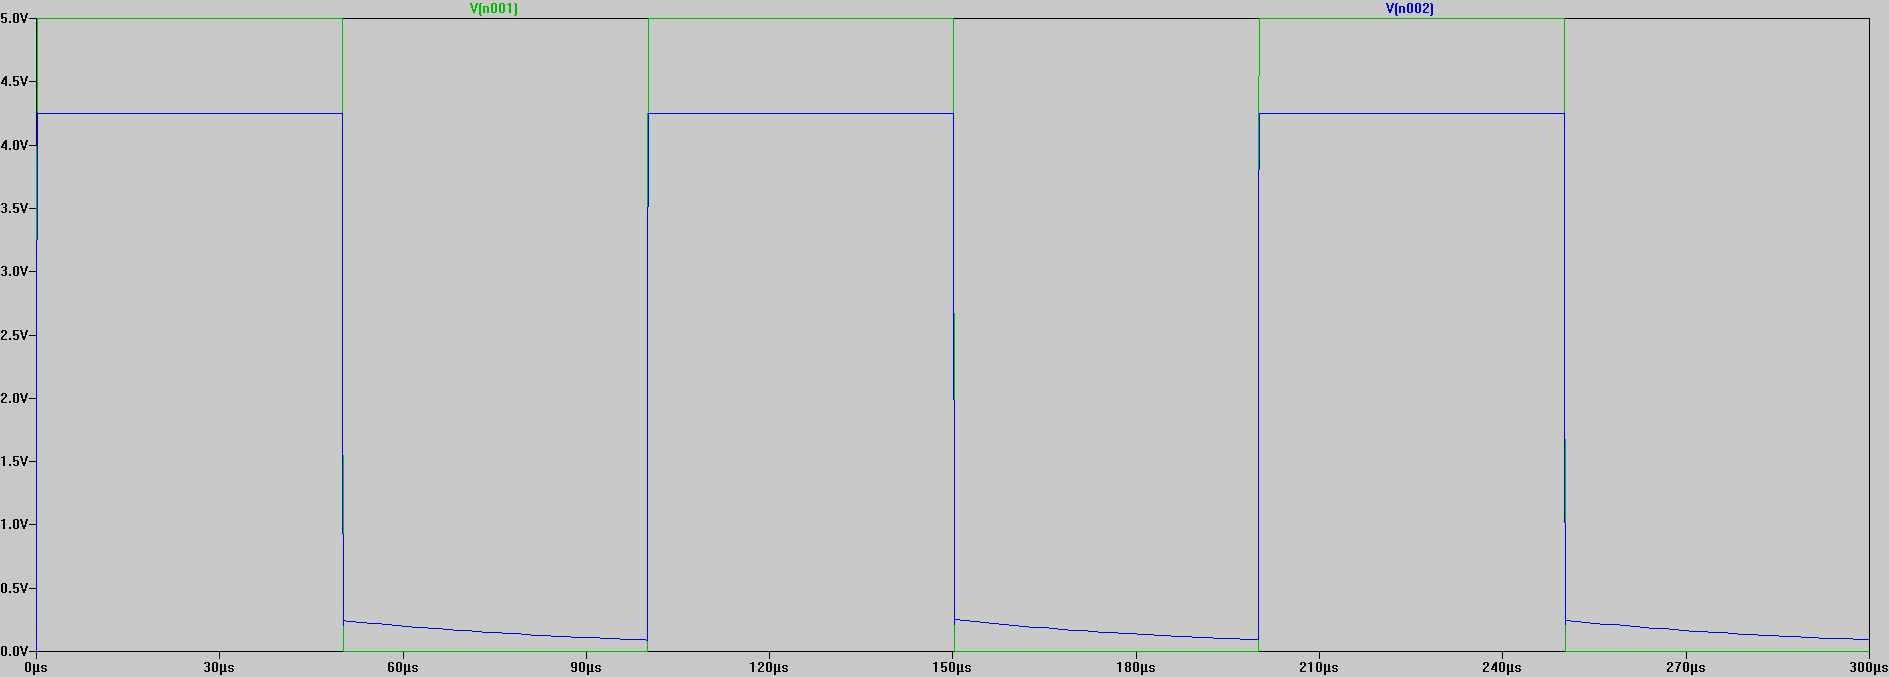
\includegraphics[width=\textwidth]{img/sim_3.png}
		\caption{C1 = 15pF, C2 = 35pF}
	\end{subfigure}
	\caption{Result running simulation for different choices of C1 and C2. Green
	curve:
	voltage of generator, blue curve: voltage at M; both compared to GND.}
	\label{fig:signal_model_result}
\end{figure}

\begin{figure}
	\centering
	\begin{tabular}{c | c}
		  Component & Capacity \\ \hline
		  1N4148PH   & 0.9pF \\
		  1N40058912 & 15pF  \\
		  LED (LTL-307GE)  & 35pF\\
	\end{tabular}
	\caption{Used components and their capacities.}
	\label{fig:signal_capacity_real} 
\end{figure}

Trying to get an idea for this behavior, a simplified model was created as
displayed in figure \ref{fig:signal_model}. The model reduces the LED to a diode. Every
diode has a small inner-capacity with the order of pF. These capacities are
added explicit in this model. The oscilloscope used to measure the voltage difference
has itself a resistance of 1M$\Omega$, which was included in the model as well.
For different choices of the the capacity C1 and C2 the circuit was simulated
and the results are shown in figure~\ref{fig:signal_model_result}.

Looking at the used components' capacities as listed in figure
\ref{fig:signal_capacity_real}, the capacities of the first and the last
simulation match the used components. While the first simulation curve matches
somewhat the shape of the measured curve in figure \ref{fig:signal_m1}, the last
simulation doesn't match the observed curve in figure \ref{fig:signal_m2}.
However, the measurement fits very well for the made-up capacities used in the
middle simulation. The reason for this remains unclear to the author.

Without adjusting the diodes D1 and D2 a rectangular wave was possible to
achieve by connecting M to GND using a resistor of 10k$\Omega$. This follows
the same idea as the resistors introduced at S, I1 and I2.

\section{Conclusion}

The experiments presented here showed some important property of digital
circuits and how to measure those. Moreover, by doing a circuit from scratch, some of
the issues designing a digital circuit were enlightened. Constructing a circuit
requires understanding all the components. Otherwise things like the
inner-capacity of diodes or the resistance of the measurement equipment might be
forgotten to be taken into account. These can lead to unexpected behavior, which
were relatively simple to hunt down in this setup, but are imagined to be
much harder to find and control on larger circuits. Given that the here
implemented circuit was simple compared to the circuits shipping with a computer/smartphone, it can only be imagined the hard work it takes to make
large circuits operate precise. 

The complexity even grows, as there are more and
more components packed on a single chip and more functionality is
covered by the same gadget. To achieve this minimization, the inner components
got smaller and smaller over the last years. This cannot continue for too long
anymore as physical limits are approached very soon. Future
improvements might require to change from the digital 
circuits to circuits using light and/or quantum states.

% THE END

\begin{comment}
\begin{center}
\line(1,0){250}
\end{center}
\end{comment}

\begin{thebibliography}{------}
\bibitem[1]{book_dg}
	U. Tietze, C. Schenk
	{\em Halbleiter-Schaltungstechnik}.
	Springer, sechste, neue Überarbeitete und erweiterte Auflage (1983), pp
	176-177
\end{thebibliography}

\end{document}
